% !TeX spellcheck = ru_RU
% !TeX encoding = UTF-8
\subsection{Технология Lora}
\subsubsection{Назначение}
Технология LoRa включает в себя метод модуляции LoRa, разработанный Semtech, и открытый протокол LoRaWAN.

Если модуляция LoRa является физическим уровнем (OSI media layer 1), то LoRaWAN (Long Range Wide-Area Networks) – это MAC протокол канального уровня (OSI media layer 2) для сетей с множеством узлов с большим радиусом действия и низким собственным потреблением мощности.   

Узлам сети характерны: низкое энергопотребление (до 10 лет работы от обычных батарей АА), невысокая скорость обмена данными, большая дальность связи (15 км в сельской местности и 5км в плотной городской застройке) и низкая стоимость оконечного оборудования.

Разработчики LoRa Alliance позиционируют LoRa как технологию, имеющую значительные преимущества перед сотовыми сетями и WiFi благодаря возможности развертывания межмашинных (M2M) коммуникаций на расстояниях до 15 км и скоростях до 50 Кбит/с, при минимальном потреблении электроэнергии, обеспечивающем несколько лет автономной работы на одном аккумуляторе типа АА.

Диапазон применений данной технологии огромен: от домашней автоматизации и интернета вещей (Internet of Things, IoT) до промышленности и умных городов.

\subsubsection{Структура системы}
Рассмотрим структуру LoRaWAN сетей. Типичная сеть LoRaWAN состоит из следующих элементов: 
\begin{itemize}
	\item"Датчики". В технологии LoRa используется термин "конечные узлы".
	\item"Приёмники". В технологии LoRa используется термин "шлюзы".
	\item"Пункт сбора". В технологии LoRa используется термин "сетевой сервер".
	\item"Облачный сервер". В технологии LoRa используется термин "сервер приложений".
\end{itemize}

Структурная схема системы представлена на рисунке
\ref{fig:LoRa}.
\begin{figure}[h]
	\centering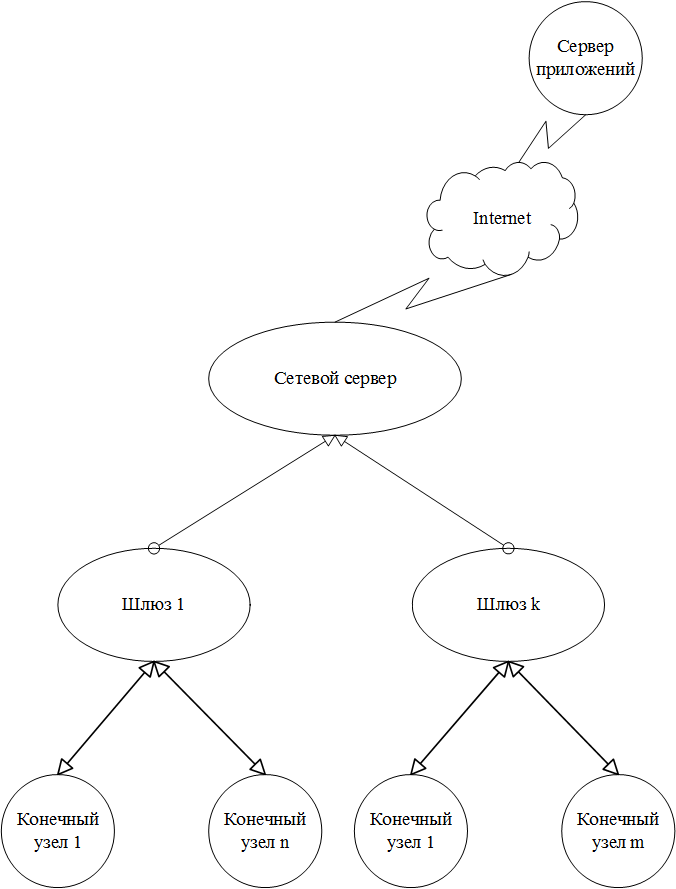
\includegraphics[width=0.7\linewidth]{img/LoRa}
	\caption{Структурная схема системы, построенной по технологии LoRa}
	\label{fig:LoRa}
\end{figure}


\textbf{Конечный узел (End Node) }предназначен для осуществления управляющих или измерительных функций. Он содержит набор необходимых датчиков и управляющих элементов.

\textbf{Шлюз LoRa (Gateway/Concentrator)} — устройство, принимающее данные от конечных устройств с помощью радиоканала и передающее их в транзитную сеть. В качестве такой сети могут выступать Ethernet, WiFi, сотовые сети и любые другие телекоммуникационные каналы. Шлюз и конечные устройства образуют сетевую топологию типа звезда. Обычно данное устройство содержит многоканальные приёмопередатчики для обработки сигналов в нескольких каналах одновременно, или даже нескольких сигналов в одном канале. Соответственно, несколько таких устройств обеспечивает зону покрытия сети и прозрачную двунаправленную передачу данных между конечными узлами и сервером.

\textbf{Сетевой сервер (Network Server)} предназначен для управления сетью: заданием расписания, адаптацией скорости, хранением и обработкой принимаемых данных.

\textbf{Сервер приложений (Application Server)} может удаленно контролировать работу конечных узлов и собирать необходимые данные с них \cite{1}.

В конечном итоге, LoRaWAN сеть имеет топологию звезда, имеет конечные узлы, которые через шлюзы, образующие прозрачные мосты, общаются с центральным сервером сети. При таком подходе обычно предполагается, что шлюзами и центральным сервером владеет оператор сети, а конечными узлами – абоненты. Абоненты имеют возможность прозрачной двунаправленной и защищенной передачи данных до конечных узлов.

Так как LoRaWAN образуют глобальную сеть, то разработчики уделили особое внимание безопасности и конфиденциальности передаваемых данных, которые обеспечиваются шифрованием AES на нескольких уровнях:



\begin{itemize}
	\item На сетевом уровне с использованием уникального ключа сети (Unique Network key, EUI64).
	\item Сквозную безопасность на уровне приложений с помощью уникального ключа приложения (Unique Application key, EUI64).
	\item И специального ключа устройства (Device specific key, EUI128).
\end{itemize}

Для решения различных задач и применений в сети LoRaWAN предусмотрено три класса устройств:

1. Двунаправленные конечные устройства «класса А» (Bi-directional end-devices, Class A). Устройства этого класса применяются, когда необходима минимальная потребляемая мощность при преобладании передачи данных к серверу. В качестве инициатора сеанса связи выступает конечный узел, отправляя пакет с необходимыми данными, а затем выделяет два окна, в течении которых ждёт данных от сервера. Таким образом, передача данных от сервера возможна только после выхода на связь конечного устройства.

2. Двунаправленные конечные устройства «класса Б» (Bi-directional end-devices, Class B). Основное отличие от устройств «класса А» заключается в выделении дополнительного окна приёма, которое устройство открывает по расписанию. Для составления расписания конечное устройство осуществляет синхронизацию по специальному сигналу от шлюза. Благодаря этому дополнительному окну сервер имеет возможность начать передачу данных в заранее известное время.

3. Двунаправленные конечные устройства «класса С» с максимальным приемным окном (Bi-directional end-devices, Class C). Устройства этого класса имеют почти непрерывное окно приёма данных и закрывают его лишь на время передачи данных, что позволяет их применять для решения задач, требующих получения большого объёма данных.

Подводя итоги, можно сказать, что LoRaWAN позволяет строить глобальные распределённые беспроводные сети с большим числом конечных узлов. По заявлениям Semtech, один LoRa-шлюз допускает обслуживание до пяти тысяч конечных устройств, что достигается за счёт:
\begin{itemize}	
\item Топологии сети.
\item Адаптивной скорости передачи данных и адаптивной выходной мощности устройств, задаваемых сетевым сервером.
\item Временным разделением доступа к среде.
\item Частотным разделением каналов.
\item Особенностью LoRa-модуляции, позволяющей в одном частотном канале одновременно демодулировать сигналы, передаваемые на разных скоростях.
\end{itemize}


\subsubsection{Разбиение системы на уровни}
Способ разбиения системы LoRa на уровни представлен на рисунке
\ref{fig:system_levels_LoRa}.
\begin{figure}[h]
	\centering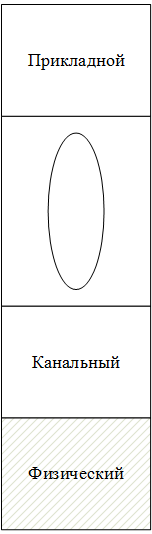
\includegraphics[width=0.2\linewidth]{img/system_levels_LoRa}
	\caption{Разбиение на уровни системы LoRa}
	\label{fig:system_levels_LoRa}
\end{figure}
\subsubsection{Особенности построения уровней}
Физический уровень системы имеет специфические особенности, так как в нем используется специальная модуляция, называемая LoRa. Модули физического уровня системы являются закрытыми.

